\section{Architektur}
\label{sec:komponenten:architektur}

Die dieser Arbeit zugrunde liegende Architektur folgt dem Ansatz von \cite{Truyen2016}, in dem eine Container basierte
Architektur für \ac{SaaS} Anwendungen vorgestellt wird. Kubernetes spielt hierbei eine wichtige Rolle. Es dient dem State
Managment, der Isolation der Workloads sowie der Authentifizierung für Tenants. Hierbei ist jeder Kontrollservice für den \ac{SaaS}
mit Kubernetes integriert.

\begin{figure}
  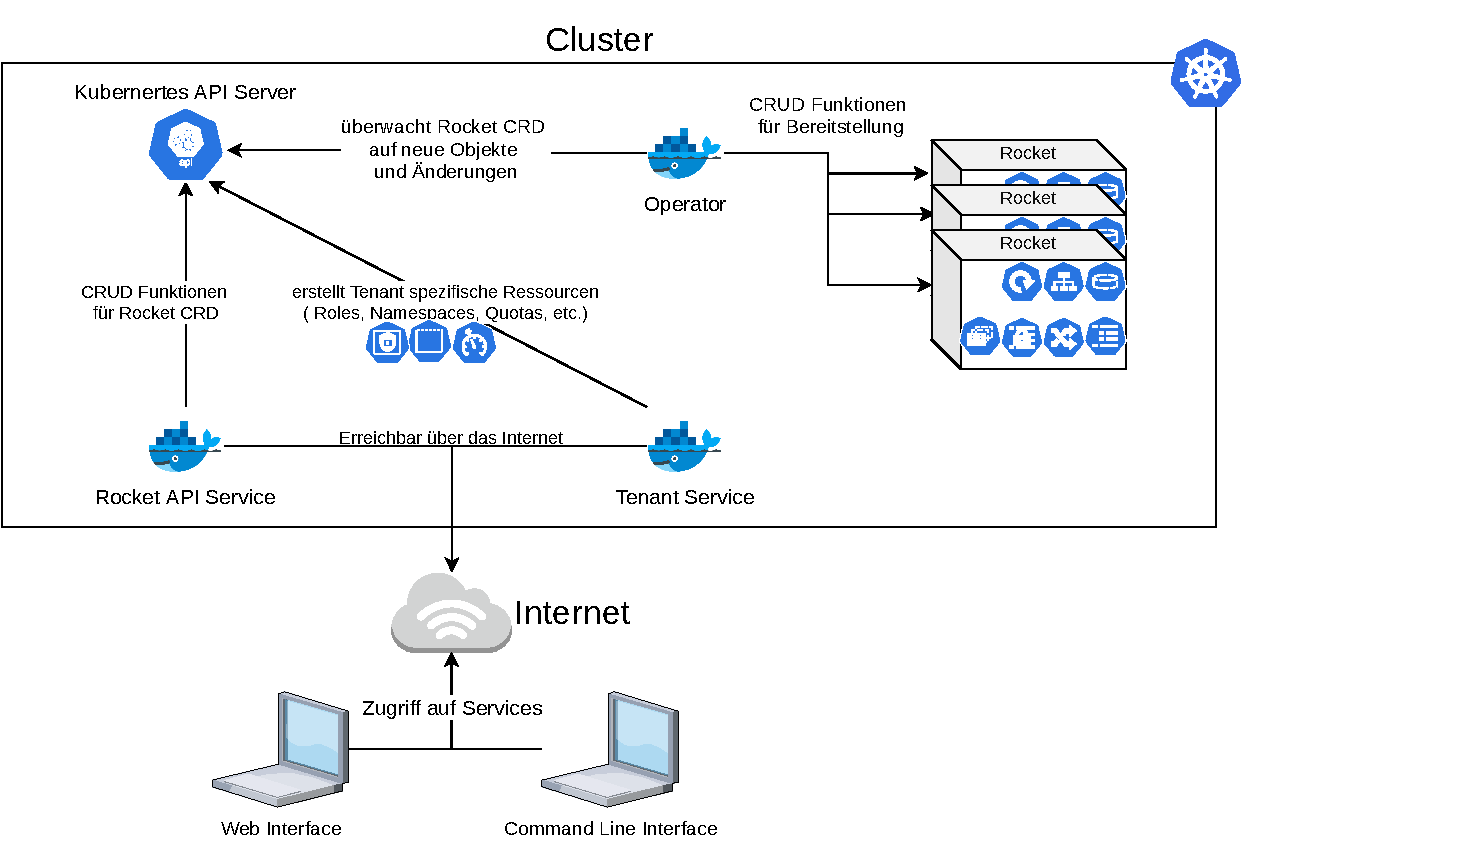
\includegraphics[width=45em]{gfx/chapters/3_komponenten/saas_architecture.pdf}
  \caption{Architektur des \ac{SaaS}}
  \label{fig:architektur}
\end{figure}

In \ref{fig:architektur} wird die Architektur nochmal bildlich dargestellt.
Hier erkennt man, dass die Hauptkomponenten der Serverseite alle mit der Kubernetes API kommunizieren,
um den gewünschten State des Clients zu erzielen. Der Operator dient als Komponente zum tatsächlichen
Erstellen der Rocket und Mongodb Container sowie Netzwerk-, Anwendungs- und Speicherkonfiguration.
% TODO: 
Der Rocket API Service hat die Aufgabe, dass vom Operator definierte \ac{CRD} im Kubernetes Cluster zu erstellen,
während der Tenant Service sich um die Konfiguration des Users im Cluster kümmert.
Hierbei werden Ressourcen wie bspw. Rollen, Namespaces und Quotas erstellt.